\documentclass[11pt]{article}
\usepackage[letterpaper,margin=0.9in]{geometry}
\usepackage{amsmath,amssymb,amsthm,mathtools}
\usepackage{booktabs,tabularx,multirow}
\usepackage{graphicx,subcaption}
\usepackage[dvipsnames]{xcolor}
\usepackage{microtype}
\usepackage{mathpazo}
\usepackage{enumitem}
\usepackage{algorithm,algpseudocode}
\usepackage[colorlinks=true,linkcolor=MidnightBlue,urlcolor=MidnightBlue,citecolor=MidnightBlue]{hyperref}
\usepackage{titlesec}
\titlespacing*{\section}{0pt}{10pt}{4pt}
\titlespacing*{\subsection}{0pt}{7pt}{3pt}
\setlist{itemsep=1pt,topsep=2pt}
\setlength{\parskip}{3pt}
\newtheorem{proposition}{Proposition}
\newcommand{\I}{\mathcal{I}}
\newcommand{\V}{\mathcal{V}}
\newcommand{\T}{\mathcal{T}}
\newcommand{\K}{\mathcal{K}}
\newcommand{\G}{\mathcal{G}}
\newcommand{\R}{\mathbb{R}}

\title{\vspace{-1.2cm}\textbf{Table for 6}\\[2pt]
\large Seating strangers across the Bay with integer programming and column generation}
\author{IEOR 240, Fall 2026 \quad\textbullet\quad [Group member names]\\
\small Video: \href{https://example.com}{[video link]} \quad\textbullet\quad Code: \href{https://github.com/amyyang027/meet-in-the-middle}{[repository link]}}
\date{}

\begin{document}
\maketitle
\vspace{-1.0cm}

\section{The problem: a city full of strangers}
\label{sec:intro}

A city is a place where you can be surrounded by 800{,}000 people and still eat dinner with your phone. Plenty of people would like to meet someone new, but the usual options are a bar (loud), an app (swiping), or a friend of a friend (finite). \emph{Table for 6} is a simpler idea: sign up, answer a short survey, and on Saturday you are at a table with five strangers at a place you would actually like, at a time you are free, without crossing the Bay Bridge at rush hour for it.

Behind that pitch is a real optimization problem. A good table needs three things at once: the \emph{place} fits everyone's taste and budget, the \emph{people} fit each other, and the \emph{trip} is short for everybody. These pull against each other. The best Ethiopian place for an Oakland vegetarian may be a 45-minute drive for the Sunset resident who would otherwise be their ideal tablemate. Random seating ignores all of this (Figure~\ref{fig:map}, left), and seating by hand stops working at about the size of a wedding.

\begin{figure}[t]
\centering
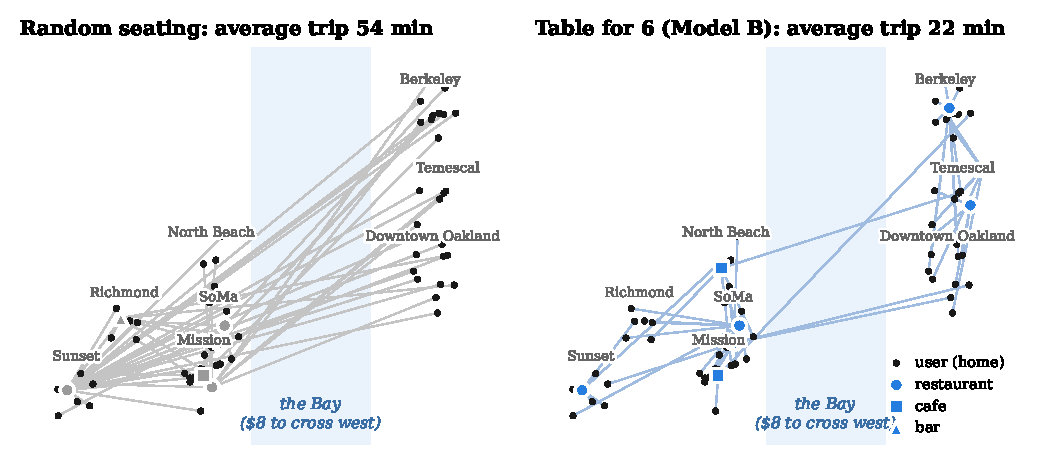
\includegraphics[width=\textwidth]{fig/map.pdf}
\vspace{-6pt}
\caption{The same 60 users and venues, seated two ways. Each line joins a user's home to their table's venue. Random seating sends people back and forth across the Bay; Model B keeps most tables on one side and cuts the average trip from 54 to 22 minutes, raises average satisfaction $p$ from 4.9 to 5.9, more than doubles average pair compatibility $q_{ij}$, and seats all 60 users instead of 57.}
\label{fig:map}
\end{figure}

\paragraph{What we built.}
\begin{enumerate}[leftmargin=*]
\item A model in which every survey answer, including age and gender, enters a satisfaction score rather than a hard filter (Section~\ref{sec:setup}).
\item \textbf{Model A}, a compact MILP built with class techniques: binary assignment variables $x_{ik}$, big-$M$ linking, and the logical AND linearization for pairs of users (Section~\ref{sec:modelA}).
\item \textbf{Model B}, a set partitioning reformulation solved by \textbf{column generation} with a certified upper bound from weak duality (Section~\ref{sec:modelB}). This is our method beyond the course.
\item Three add-ons the group agreed on: a fairness floor, table diversity, and robustness to no-shows. The last one is only expressible exactly in Model B (Section~\ref{sec:addons}).
\item Experiments on synthetic Bay Area data comparing random seating, a greedy heuristic, Model A, and Model B (Section~\ref{sec:results}).
\end{enumerate}

\section{Setup and data}
\label{sec:setup}

\paragraph{Sets.} Users $i,j\in\I$ with $|\I|=N$; venues $v\in\V$ (restaurants, cafes, and bars); time slots $t\in\T=\{\text{Fri 7pm},\ \text{Sat 11am},\ \text{Sat 7pm}\}$. Venue $v$ can host $R_{vt}\in\{0,1,2\}$ tables in slot $t$, with $R_{vt}=0$ when it is closed (cafes are closed at night, bars in the morning). A \emph{candidate table} $k\in\K$ is one of the $R_{vt}$ copies of an open pair $(v,t)$, and we write $v(k)$ and $t(k)$ for its venue and slot. Fixing the venue and slot of each candidate table in advance is the key modeling choice: travel and tolls become constants for each user and table, so the model stays linear. This mirrors the hospital matching example from lecture, where we use binary $x_{ij}$ rather than a variable that holds a hospital label.

\paragraph{User-to-table satisfaction.} For user $i$ at venue $v$ in slot $t$,
\begin{equation}
p_{ivt} = w_1\,m^{\text{type}}_{iv} + w_2\,m^{\text{cuisine}}_{iv} + w_3\,m^{\text{price}}_{iv} + w_4\,m^{\text{slot}}_{it},
\end{equation}
where each match score $m\in[0,1]$ comes from a survey answer (for example $m^{\text{type}}_{iv}=(\text{rating}_{i,\text{type}(v)}-1)/4$ on a 1--5 scale) and $w=(3.5,3.5,1.5,1.5)$, so $p_{ivt}\in[0,10]$. Subtracting the cost of getting there gives the net value
\begin{equation}
c_{ik} = p_{i\,v(k)\,t(k)} - \lambda_d\, d_{i\,v(k)\,t(k)} - \lambda_\tau\, \tau_{i\,v(k)},
\end{equation}
with travel time $d_{ivt}$ in minutes, toll $\tau_{iv}$ in dollars, $\lambda_d=0.08$ per minute, and $\lambda_\tau=0.20$ per dollar. In words, 25 minutes of travel costs as much as a cuisine you rate 1 instead of 5, and an \$8 bridge toll costs 1.6 points.

\paragraph{Pairwise compatibility.} For two users $i\neq j$,
\begin{equation}
q_{ij} = \beta_1\cos(\mathbf{h}_i,\mathbf{h}_j) - \beta_2\,\frac{|\text{age}_i-\text{age}_j|}{10} + \beta_3\, g_{ij},
\qquad \beta=(3.0,\,1.5,\,0.8),
\end{equation}
where $\mathbf{h}_i\in\{0,1\}^{15}$ is user $i$'s interest vector (hiking, board games, jazz, and so on) and $g_{ij}$ is the gender-mixing term. By default $g_{ij}=1$ if $i$ and $j$ differ in gender and $0$ otherwise, so the model leans toward mixed tables. If either user asked for a same-gender table, the sign flips: $g_{ij}=1$ for a same-gender pair and $-1$ otherwise. Gender is therefore a weight that users can steer, never a filter. Note that $q_{ij}$ can be negative.

\paragraph{Feasibility.} Availability $a_{it}\in\{0,1\}$ is the only hard rule about users: user $i$ is never seated in a slot they cannot attend. Tables have between $L=4$ and $U=6$ people.

\paragraph{Synthetic data.} Our group can run a survey later, but for now every instance comes from a generator that samples users and venues around eight Bay Area neighborhoods (five in San Francisco, three in the East Bay). Ages are roughly normal around 28; interests come from five latent ``personas'' so that compatible people actually exist; 55\% of users drive and the rest take transit. Travel time is $1.35\times$ the straight-line distance at 24 km/h by car or 17 km/h by transit, plus 6 minutes to park or walk. A trip across the bay goes through the Bay Bridge, with 5--15 extra minutes depending on the slot, and drivers heading west into San Francisco pay an \$8 toll. The generator scales the number of venues with $N$ (about $N/6$) so that capacity is tight but feasible. Appendix~\ref{app:params} lists every parameter.

\section{Model A: a compact MILP}
\label{sec:modelA}

\paragraph{Decision variables.}
$x_{ik}\in\{0,1\}$ is $1$ if user $i$ sits at table $k$ (defined only when $a_{i\,t(k)}=1$);
$z_k\in\{0,1\}$ is $1$ if table $k$ opens;
$y_{ijk}\in[0,1]$ for $i<j$ is $1$ if users $i$ and $j$ both sit at table $k$;
$u_i\in\{0,1\}$ is $1$ if user $i$ is not seated this round;
$\overline{A}_k,\underline{A}_k\ge 0$ are the oldest and youngest ages at table $k$, and $e_k\ge 0$ is the age spread above $\bar{A}=12$ years.

\paragraph{Objective.} Maximize total satisfaction net of travel, plus pair compatibility, minus a penalty $M=8$ for every user left out and a penalty $\kappa=0.5$ per year of age spread beyond $\bar A$:
\begin{equation}
\max\quad \sum_{i\in\I}\sum_{k\in\K} c_{ik}\,x_{ik} \;+\; \sum_{k\in\K}\sum_{i<j} q_{ij}\,y_{ijk} \;-\; M\sum_{i\in\I}u_i \;-\; \kappa\sum_{k\in\K} e_k .
\label{eq:objA}
\end{equation}

\paragraph{Constraints.}
\begin{alignat}{3}
&\textstyle\sum_{k\in\K} x_{ik} + u_i = 1 &\qquad& \forall\, i\in\I &\qquad& \text{sit once or be left out} \label{eq:assign}\\
&L\,z_k \le \textstyle\sum_{i\in\I} x_{ik} \le U\,z_k && \forall\, k\in\K && \text{4 to 6 at an open table} \label{eq:size}\\
&y_{ijk}\le x_{ik},\quad y_{ijk}\le x_{jk} && \forall\, i<j,\ k && \text{pair only if both sit there} \label{eq:and1}\\
&y_{ijk}\ge x_{ik}+x_{jk}-1 && \forall\, i<j,\ k:\ q_{ij}<0 && \text{a bad pair cannot hide} \label{eq:and2}\\
&\overline{A}_k \ge \text{age}_i\,x_{ik},\quad \underline{A}_k \le \text{age}_i + A^{\max}(1-x_{ik}) && \forall\, i,k && \text{age range} \label{eq:age}\\
&e_k \ge \overline{A}_k - \underline{A}_k - \bar A - A^{\max}(1-z_k) && \forall\, k && \text{age spread} \\
&z_k \le z_{k-1} && \text{copies of one } (v,t) && \text{symmetry breaking} \label{eq:sym}
\end{alignat}
Constraint~\eqref{eq:size} is the big-$M$ linking pattern from lecture with $M=U$: no one can sit at a closed table, and an open table cannot have 1--3 people. Constraints~\eqref{eq:and1}--\eqref{eq:and2} are the logical AND trick: $y_{ijk}=x_{ik}x_{jk}$ at any integer point. When $q_{ij}>0$ the solver already wants $y_{ijk}$ as large as possible, so only the upper bounds are needed. Venue capacity $R_{vt}$ is built into $\K$, which has exactly $R_{vt}$ copies of $(v,t)$, and~\eqref{eq:sym} stops the solver from exploring copies that are just relabelings of each other.

\paragraph{Why Model A does not scale.} Model A is correct, but it is large and has a weak LP relaxation. With $N$ users and $|\K|$ tables there are $O(N^2|\K|)$ pair variables. At $N=60$ and $|\K|\approx 40$, that is about 70{,}000 $y_{ijk}$. Worse, the LP relaxation can set every $x_{ik}=1/|\K|$ and every $y_{ijk}$ to the same small fraction, so the bounds that branch and bound relies on are far from the truth. Branch and bound then has to work hard just to prove what it already found.

\section{Model B: choose whole tables with column generation}
\label{sec:modelB}

\paragraph{Set partitioning reformulation.} Instead of seating people one at a time, choose whole tables. A \emph{column} $g$ is one complete table: a member set $S_g\subseteq\I$ with $L\le|S_g|\le U$, a venue $v_g$, and a slot $t_g$ that every member can attend. Let $\G$ be the set of all such tables, and $\G_{vt}\subseteq\G$ the tables at $(v,t)$. Each member's value at table $g$ splits the pair terms evenly,
\begin{equation}
U_{ig} = c_{i\,v_g t_g} + \tfrac12\textstyle\sum_{j\in S_g\setminus\{i\}} q_{ij},
\qquad
C_g = \textstyle\sum_{i\in S_g} U_{ig} - \kappa\, e_g ,
\end{equation}
where $e_g$ is table $g$'s age spread above $\bar A$. With $\lambda_g\in\{0,1\}$ for choosing table $g$ and $A_{ig}=1$ if $i\in S_g$, the master problem is
\begin{align}
\max\quad & \textstyle\sum_{g\in\G} C_g\,\lambda_g - M\sum_{i\in\I} u_i \label{eq:master}\\
\text{s.t.}\quad & \textstyle\sum_{g\in\G} A_{ig}\,\lambda_g + u_i = 1 && \forall\, i\in\I && (\text{dual } \pi_i\ \text{free}) \notag\\
& \textstyle\sum_{g\in\G_{vt}} \lambda_g \le R_{vt} && \forall\, (v,t) && (\text{dual } \mu_{vt}\ge 0). \notag
\end{align}
Every nonlinear piece of Model A (pairs, age range) is now inside the constant $C_g$. That is the main advantage: any rule about a whole table can be checked by computing a number, not by adding variables. The catch is that $|\G|$ is enormous. With $N=60$ users, about 36 of whom are free in a typical slot, there are roughly 2.3 million possible groups of four to six people at each $(v,t)$.

\paragraph{Column generation.} We never write down all of $\G$. We start with a few columns, then add only the ones that can help:
\begin{enumerate}[leftmargin=*]
\item \textbf{Restricted master.} Solve the LP relaxation of~\eqref{eq:master} ($0\le\lambda_g\le1$) over the current columns $\G'\subseteq\G$, starting from the greedy solution's tables.
\item \textbf{Duals.} Read the optimal duals: $\pi_i$ is what seating user $i$ is currently worth, and $\mu_{vt}$ is the shadow price of one more table at $(v,t)$.
\item \textbf{Pricing.} For each $(v,t)$, look for a table with positive \emph{reduced cost}. As in Lecture 16, the reduced cost of a column is its objective coefficient minus $a_g^\top y^*$:
\begin{equation}
\bar{C}_g = C_g - \textstyle\sum_{i\in S_g}\pi_i - \mu_{v_g t_g}
= \sum_{i\in S_g}\bigl(c_{i v_g t_g} - \pi_i\bigr) + \sum_{\substack{i<j\\ i,j\in S_g}} q_{ij} - \kappa e_g - \mu_{v_g t_g}.
\label{eq:redcost}
\end{equation}
In a maximization LP, a column with $\bar C_g>0$ would improve the objective if it entered the basis.
\item \textbf{Repeat or stop.} Add every column with $\bar C_g>0$ and return to step 1. When pricing finds none, the restricted master LP is optimal for the full LP over all of $\G$.
\item \textbf{Integer solution.} Solve~\eqref{eq:master} as an IP over the generated columns with HiGHS branch and bound. This is called \emph{price-and-branch}.
\end{enumerate}

\paragraph{The pricing problem.} Maximizing~\eqref{eq:redcost} over $S\subseteq\{i: a_{it}=1\}$ with $L\le|S|\le U$ is a cardinality-constrained quadratic knapsack problem. It is Model A for a single table, with the duals folded into the weights. We solve it two ways. A fast heuristic grows a table greedily from several seed users and then improves it by swapping, adding, or dropping one member at a time (Algorithm~\ref{alg:pricing} in the appendix). The exact version is a small MILP with $b_i\in\{0,1\}$, the AND linearization on $b_ib_j$, and the same age-range constraints as~\eqref{eq:age}. We use the heuristic in every iteration and the exact MILP only once at the end, to prove that no improving column is left.

\paragraph{A certified bound from weak duality.}
\begin{proposition}
Let $(\pi,\mu)$ be the optimal duals of the restricted master, and let $\bar r_{vt}$ be any upper bound on $\max_{g\in\G_{vt}} \bar C_g$. Then
\begin{equation}
z^{\text{IP}} \;\le\; z^{\text{LP}} \;\le\; \textstyle\sum_{i\in\I}\pi_i + \sum_{(v,t)} R_{vt}\bigl(\mu_{vt}+\max\{0,\bar r_{vt}\}\bigr).
\label{eq:ub}
\end{equation}
\end{proposition}
\begin{proof}[Sketch]
Raising each $\mu_{vt}$ to $\mu_{vt}+\max\{0,\bar r_{vt}\}$ makes every column's reduced cost nonpositive, so the shifted duals are feasible for the dual of the full LP. The column $u_i$ stays dual feasible because it is in every restricted master. By weak duality (Lectures 5--6), the dual objective at any dual feasible point bounds the primal LP, and the LP bounds the IP.
\end{proof}
\noindent When exact pricing proves $\bar r_{vt}\le 0$ everywhere, the bound equals $z^{\text{LP}}$ and the gap $(\text{UB}-z^{\text{IP}})/\text{UB}$ is a certificate of near-optimality, the same idea as pruning by bound in branch and bound.

\subsection{Add-ons}
\label{sec:addons}

\paragraph{Fairness floor.} Maximizing the total can hand one person a bad table so that five others do slightly better. We add a variable $\theta$, the worst seated user's value, and reward it:
\begin{equation}
\max\ \eqref{eq:master} + \gamma\,\theta
\quad\text{s.t.}\quad
\theta \le \textstyle\sum_{g\in\G} U_{ig}\,\lambda_g - M\,u_i \quad \forall\, i\in\I \quad(\text{dual } \sigma_i\ge 0),
\end{equation}
so an unseated user counts as value $-M$ (which also stops the solver from ``protecting'' people by not seating them). This is the max-min idea from class, and it fits column generation cleanly: the reduced cost becomes $\bar C_g = \sum_{i\in S_g}\bigl[(1+\sigma_i)U_{ig}-\pi_i\bigr]-\kappa e_g-\mu_{v_gt_g}$, which is the same pricing problem with reweighted users.

\paragraph{Table diversity.} The gender-mixing term $g_{ij}$ in $q_{ij}$ and the age-spread penalty $\kappa e_g$ together keep tables from being either a monoculture or a random mix of 22- and 45-year-olds.

\paragraph{Robustness to no-shows.} If user $i$ shows up with probability $\phi_i$ (independently), a table of four collapses when anyone flakes. In Model A the best we can do is a linear proxy on expected attendance, $\sum_i\phi_i x_{ik}\ge E\,z_k$ with $E=4.25$. In Model B we can enforce the exact \emph{chance constraint} for each column,
\begin{equation}
\Pr\Bigl(\textstyle\sum_{i\in S_g}\xi_i\ge L\Bigr)\ge \alpha,\qquad \xi_i\sim\text{Bernoulli}(\phi_i),\ \alpha=0.9,
\end{equation}
by computing the Poisson-binomial distribution of attendance with a short dynamic program and discarding any table that fails. This constraint is nonlinear in $x$, so Model A cannot express it. In Model B it costs one function call per candidate table.

\section{Results}
\label{sec:results}

We compare four methods: \textbf{Random} (shuffle users into open tables, the ``seating chart drawn by a cat''), \textbf{Greedy} (repeatedly open the best table per seat), \textbf{Model A} (HiGHS on the compact MILP), and \textbf{Model B} (column generation). All runs use one CPU thread. Quality is measured against the certified upper bound~\eqref{eq:ub}, so a gap of $0\%$ means provably optimal.

\subsection{Quality: Model B is near-optimal, and provably so}

\begin{table}[h]
\centering\small
\begin{tabular}{@{}r rrrr rr@{}}
\toprule
& \multicolumn{4}{c}{Gap to upper bound (\%)} & \multicolumn{2}{c}{Seconds} \\
\cmidrule(lr){2-5}\cmidrule(l){6-7}
$N$ & Random & Greedy & Model A & Model B & Model A & Model B \\
\midrule
12 & 94.7 & 38.1 & 0.7 & 0.7 & 10.6 & 1.8 \\
18 & 106.9 & 23.2 & 0.9 & 1.2 & 26.8 & 4.8 \\
24 & 76.0 & 24.1 & 2.1 & 0.8 & 90.2 & 9.7 \\
30 & 78.0 & 19.9 & 8.7 & 0.9 & 90.3 & 41.6 \\
\bottomrule
\end{tabular}
\caption{Small instances. Model A gets a 90-second limit per instance. For $N\le 18$ it finishes, and Model B matches its proven optimum in 9 of 10 instances. For $N\ge 24$ Model A hits the time limit every time, while Model B stays within about 1\% of the bound in seconds.}
\label{tab:e1}
\end{table}

Table~\ref{tab:e1} and Figure~\ref{fig:qsc}a tell a consistent story. Random seating is not just bad but often \emph{negative}: it strands people who cannot make the slot it picked and seats others an hour from home. Greedy is far better but myopic. It fills the most attractive tables first and leaves 6--13\% of users with no feasible table at the end (Model B seats everyone in 19 of 20 instances). Model A is exact when it finishes, and it is the reason we trust the comparison: on the ten instances with $N\le18$, Model B equals Model A's proven optimum nine times and is 2\% short once. That one miss is the price of solving the final IP only over generated columns (``price-and-branch'') rather than generating columns inside every branch-and-bound node. From $N=24$ on, Model A runs out of time with gaps up to 13\%, while Model B finishes in 5--40 seconds and never exceeds a 1.9\% gap.

\subsection{Scale: the compact MILP stalls, column generation does not}

\begin{figure}[t]
\centering
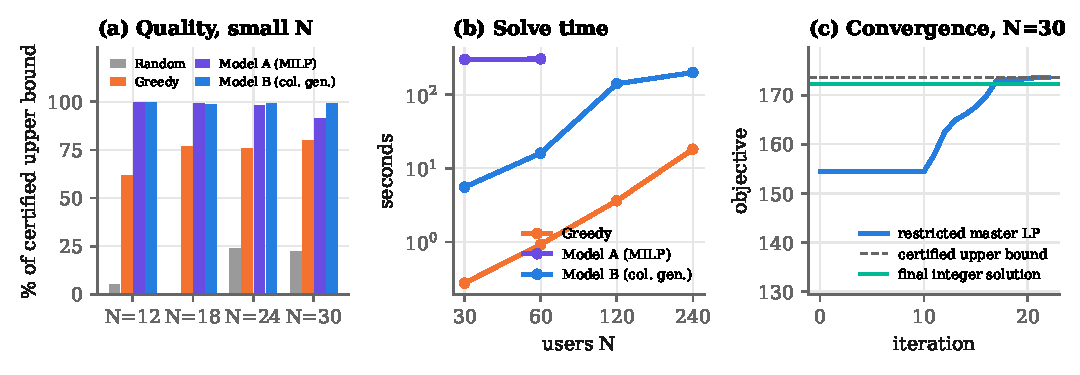
\includegraphics[width=\textwidth]{fig/quality_scale_cg.pdf}
\vspace{-14pt}
\caption{(a) Share of the certified upper bound achieved, averaged over 5 instances per $N$ (Random averages between $-7\%$ and $24\%$; a negative average is drawn at 0). (b) Mean solve time; Model A is stopped at 300 seconds. (c) One run of column generation at $N=30$: the restricted master LP climbs to the full LP optimum in 22 iterations using 312 of the roughly 350{,}000 possible tables, and exact pricing then certifies it as an upper bound.}
\label{fig:qsc}
\end{figure}

Figure~\ref{fig:qsc}b shows solve times up to $N=240$. Model A has $O(N^2|\K|)$ pair variables, over 5{,}000 variables in total at $N=30$, and its LP relaxation gives branch and bound little to prune with. At $N=60$, after 300 seconds, its best seating is worth only about 76\% of Model B's, which Model B finds in about 15 seconds. Model B's time grows because both the number of $(v,t)$ pairs and the pricing pool grow with $N$, but it still seats 240 users in about 3.5 minutes and beats Greedy by 9.5\% on average across $N\ge60$. The advantage shrinks with size, from 8--18\% at $N=60$ to 5--6\% at $N=240$, and Model B's own gap to its LP value grows from under 1\% to about 4\%. At that size our integer step (pool IP plus diving) becomes the bottleneck, which is the first thing full branch-and-price would fix.

Figure~\ref{fig:qsc}c shows column generation at work. The first restricted master contains only the greedy tables. Each round of pricing uses the duals $\pi_i$ and $\mu_{vt}$ to find tables with positive reduced cost~\eqref{eq:redcost}. The LP value rises quickly and then flattens. Exact pricing then finds no improving column, so the LP value \emph{is} the bound, and the integer solution is within 0.75\% of it.

\subsection{What the add-ons buy}

\begin{figure}[t]
\centering
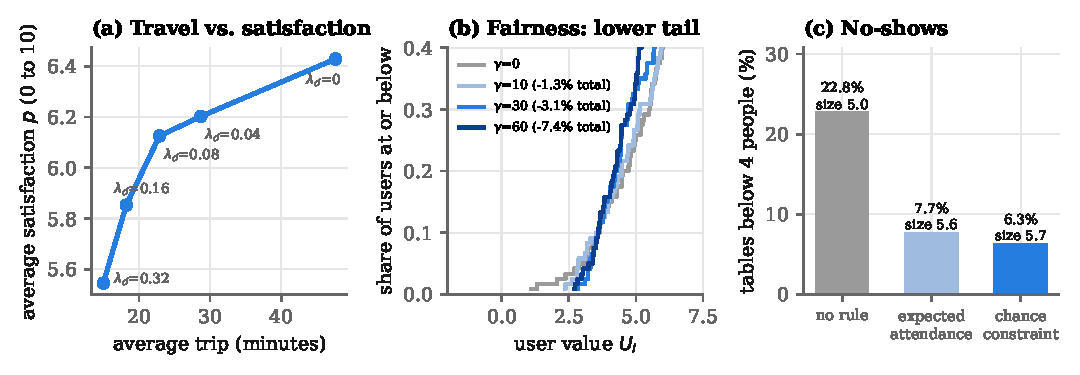
\includegraphics[width=\textwidth]{fig/tradeoffs.pdf}
\vspace{-14pt}
\caption{Trade-offs at $N=60$ (Model B). (a) Raising the value of time $\lambda_d$ shortens trips much faster than it lowers satisfaction, until $\lambda_d=0.32$. (b) Distribution of user value $U_i$, lower tail only: the fairness floor lifts the worst-off users from about $-0.5$ to about $4$ for a 1--3\% drop in total value. (c) Share of tables that drop below four people in 5{,}000 simulated evenings, with the average table size above each bar.}
\label{fig:trade}
\end{figure}

\paragraph{Travel.} In Figure~\ref{fig:trade}a, moving from $\lambda_d=0$ (travel is free) to our default $\lambda_d=0.08$ cuts the average trip from 50 to 23 minutes, a 54\% drop, while average satisfaction $p$ falls only from 6.29 to 6.00 out of 10. The share of users paying a bridge toll falls from 5\% to under 1\%. The curve bends sharply after $\lambda_d=0.16$: squeezing trips below 19 minutes starts sending people to places they do not like. This is the shadow-price way to read $\lambda_d$: it is the exchange rate between a minute and a point of satisfaction, and the knee tells us where the exchange gets expensive.

\paragraph{Fairness.} With $\gamma=0$ the solver happily gives a few users a value near zero to help everyone else. A modest weight $\gamma=10$ raises the worst user's value $\theta$ from $-0.45$ to $3.9$ on average and costs only 1.2\% of total value (Figure~\ref{fig:trade}b). Larger $\gamma$ buys little extra floor for more cost. In the reduced cost this appears as the reweighting $(1+\sigma_i)$: users with a positive fairness dual $\sigma_i$ become more valuable to seat well.

\paragraph{No-shows.} With no rule, 15.3\% of tables lose enough people to fall below four (Figure~\ref{fig:trade}c). The linear proxy in Model A, expected attendance $\sum_i\phi_i x_{ik}\ge 4.25$, cuts this to 5.7\%. The exact chance constraint with $\alpha=0.9$, available only in Model B, cuts it to 4.2\% and guarantees that \emph{every} table's risk is below 10\%, which the proxy cannot promise (on one instance the proxy's tables averaged an 8.4\% risk). Both rules work mostly by making tables bigger, and they cost about 1.0\% and 1.5\% of planned value.

\section{Discussion}
\label{sec:discussion}

\paragraph{What worked and why.} Column generation wins for two reasons. First, the set partitioning LP is much tighter than Model A's LP: in Model A a fractional user can be ``a sixth at every table,'' while in Model B the LP can only mix whole, sensible tables. A tighter relaxation means better bounds, which is exactly what branch and bound needs. Second, every table-level rule, including the pairs, the age range, and the nonlinear chance constraint, becomes a number computed once per column instead of new variables and big-$M$ constraints. Duals and reduced costs, which in class we used mainly to read sensitivity off a final tableau, here drive the whole algorithm.

\paragraph{Limitations.} (1) Our integer step is price-and-branch, not full branch-and-price, so Model B is not guaranteed optimal; it was 2\% short in one small case. (2) Exact pricing is a quadratic knapsack MILP, and beyond about 30 users it is too slow to run to completion, so for large $N$ we report the gap to the LP value under heuristic pricing, which is not a certified bound. (3) The data are synthetic, and the travel model (a fixed detour factor, a constant speed, and one bridge) is crude. (4) No-shows are assumed independent; friends who cancel together would break that.

\paragraph{Next steps.} The obvious next step is a short survey of real users to replace the generator; the model needs no change, only new values of $p_{ivt}$ and $q_{ij}$. On the methods side, branching on pairs (``$i$ and $j$ together or apart,'' the Ryan--Foster rule) would turn price-and-branch into exact branch-and-price. Finally, a weekly version could set $q_{ij}=-\infty$ for pairs who have already met, so the city keeps getting a little smaller. After that, \emph{Table for 6} becomes a product: we already have a Streamlit and HiGHS stack from our first prototype, and the solver is fast enough to run while someone waits for their coffee.


\clearpage
\appendix
\section*{Appendix}
\addcontentsline{toc}{section}{Appendix}

\section{Notation and parameter values}
\label{app:params}

\begin{table}[h]
\centering\small
\begin{tabularx}{\textwidth}{@{}l X l@{}}
\toprule
Symbol & Meaning & Value in experiments \\
\midrule
$\I$, $N$ & users & $N\in\{12,\dots,240\}$ \\
$\V$ & venues (restaurant, cafe, bar) & $\lceil N/6\rceil$, at least 8; 50/25/25\% by type \\
$\T$ & time slots & Fri 7pm, Sat 11am, Sat 7pm \\
$R_{vt}$ & tables venue $v$ can host in slot $t$ & 1 or 2 when open, 0 when closed \\
$\K$, $v(k)$, $t(k)$ & candidate tables and their venue and slot & $R_{vt}$ copies of each open $(v,t)$ \\
$a_{it}$ & 1 if user $i$ can attend slot $t$ & each slot w.p.\ 0.6, at least one \\
$p_{ivt}$ & user-to-table satisfaction, in $[0,10]$ & $w=(3.5,3.5,1.5,1.5)$ \\
$d_{ivt}$, $\tau_{iv}$ & travel minutes and toll dollars & see Section~\ref{sec:setup}; toll \$8 westbound \\
$\lambda_d$, $\lambda_\tau$ & value of a minute and of a dollar & $0.08$, $0.20$ \\
$c_{ik}$ & net value of user $i$ at table $k$ & $p-\lambda_d d-\lambda_\tau\tau$ \\
$q_{ij}$ & pairwise compatibility & $\beta=(3.0,1.5)$; range about $[-3.2,2.9]$ \\
$\ell_i$, $\Q$ & gender of user $i$; users who asked for a same-gender table & 48/48/4\% W/M/NB; 12\% ask \\
$L$, $U$ & table size limits & 4, 6 \\
$M$ & penalty for an unseated user & 8 \\
$\bar A$, $\kappa$ & allowed age spread and penalty per extra year & 12 years, 0.5 \\
$\gamma$ & weight on the fairness floor $\theta$ & $0$ unless stated \\
$\phi_i$ & probability that user $i$ shows up & Beta$(8.5,1.5)$, clipped to $[0.55,0.99]$, mean 0.85 \\
$E$, $\alpha$ & expected-attendance floor and chance level & 4.25, 0.9 \\
$\pi_i$, $\mu_{vt}$, $\sigma_i$ & master duals (partition, capacity, fairness) & from HiGHS \\
\bottomrule
\end{tabularx}
\end{table}

\section{Pricing heuristic}

\begin{algorithm}[h]
\caption{Heuristic pricing at $(v,t)$ with weights $w_i=(1+\sigma_i)c_{ivt}-\pi_i$ and $\hat q_{ij}=\tfrac12(2+\sigma_i+\sigma_j)q_{ij}$}
\label{alg:pricing}
\begin{algorithmic}[1]
\State $P\gets\{i: a_{it}=1\}$; seeds $\gets$ the 6 users with the largest $w_i$, plus 3 random users
\For{each seed $s$}
  \State $S\gets\{s\}$; \textbf{while} $|S|<U$: add $\arg\max_{j\in P\setminus S}\ \bigl(w_j+\sum_{i\in S}\hat q_{ij}\bigr)$
  \State keep the best feasible prefix of size $L,\dots,U$ (feasible: availability, and the no-show rule if on)
  \Repeat \Comment{best-improvement local search}
    \State evaluate every swap $(a\in S,\ b\notin S)$, every add, and every drop, using
    \Statex \hspace{\algorithmicindent} $\Delta(a\to b)=w_b+\sum_{j\in S}\hat q_{bj}-\hat q_{ab}-w_a-\sum_{j\in S}\hat q_{aj}$, then the exact age penalty
    \State move to the best feasible improving neighbor
  \Until{no move improves}
\EndFor
\State \Return the best tables whose reduced cost $\bar C_g$ is positive
\end{algorithmic}
\end{algorithm}

\noindent After column generation stops, two cheap steps produce the integer solution. First, we enrich the column pool with every drop-one subset of each generated table and every generated group moved to another open $(v,t)$, then solve the master IP over the pool. Second, a \emph{diving} heuristic repeatedly fixes the table with the largest LP value $\lambda_g$, removes its members from pricing, and re-runs column generation on what is left. We keep the better of the two.

\section{Code}
All code is in Python 3.13 with HiGHS 1.16 (through \texttt{highspy}, and \texttt{PuLP} 2.9 for Model A).
\begin{itemize}
\item \texttt{t6/data.py}: synthetic instance generator and all parameters $p$, $c$, $q$, $d$, $\tau$.
\item \texttt{t6/solve.py}: random and greedy baselines, Model A, the restricted master, heuristic and exact pricing, the weak-duality bound, pool enrichment, and diving.
\item \texttt{experiments/run.py}: experiments E1 to E5; \texttt{experiments/figures.py}: every figure in this report.
\end{itemize}
Every experiment uses fixed random seeds, so \texttt{python -m experiments.run e1} reproduces Table~\ref{tab:e1} exactly (up to solver time limits).


\end{document}
